\documentclass[a4paper]{article}

\title{PH2255 Course:\\
Quantum Harmonic Oscillators}
\author{Thomas Bass}
\date{27 March 2021}

% LaTeX preambule: loading relevant packages, configuring Python listings
\usepackage{graphicx}
\usepackage{amsmath}
\usepackage{color}
\usepackage{listings}
\usepackage{hyperref}
\usepackage{bm}
\usepackage{physics}
\usepackage[a4paper, total={6in, 8in}]{geometry}

\definecolor{dkgreen}{rgb}{0,0.6,0}
\definecolor{gray}{rgb}{0.5,0.5,0.5}
\definecolor{mauve}{rgb}{0.58,0,0.82}

% Settings for colour-coding and formatting Python code:
\lstset{
  language=Python,                % the language of the code
  basicstyle=\footnotesize,           % the size of the fonts that are used for the code
  numbers=left,                   % where to put the line-numbers
  numberstyle=\tiny\color{gray},  % the style that is used for the line-numbers
  stepnumber=5,                   % the step between two line-numbers. If it's 1, each line
                                  % will be numbered
  numbersep=5pt,                  % how far the line-numbers are from the code
  backgroundcolor=\color{white},      % choose the background color. You must add \usepackage{color}
  showspaces=false,               % show spaces adding particular underscores
  showstringspaces=false,         % underline spaces within strings
  showtabs=false,                 % show tabs within strings adding particular underscores
  frame=single,                   % adds a frame around the code
  rulecolor=\color{black},        % if not set, the frame-color may be changed on line-breaks within not-black text (e.g. commens (green here))
  tabsize=2,                      % sets default tabsize to 2 spaces
  captionpos=b,                   % sets the caption-position to bottom
  breaklines=true,                % sets automatic line breaking
  breakatwhitespace=false,        % sets if automatic breaks should only happen at whitespace
  title=\lstname,                   % show the filename of files included with \lstinputlisting;
                                  % also try caption instead of title
  keywordstyle=\color{blue},          % keyword style
  commentstyle=\color{dkgreen},       % comment style
  stringstyle=\color{mauve},         % string literal style
  escapeinside={\%*}{*)},            % if you want to add LaTeX within your code
  morekeywords={*,...}               % if you want to add more keywords to the set
}

\begin{document}
\maketitle

\begin{abstract}
%%%%%%
TODO
%%%%%%
\end{abstract}

\section{Hooke's Law and the Quantum Harmonic Oscillator}
To begin an analysis of quantum harmonic oscillators, we begin with Hooke's law. While this law is in the classical regime, later it can be proved - with Bohr's correspondence principle - that we can apply the same potentials described by Hooke's spring model to the forces experienced by an atom in equilibrium. Just as Hooke's law describes the force on a mass displaced from its equilibrium, here we use it to describe the potential gained by a quantum object in terms of its angular frequency. By differentiating Hooke's law we can obtain the work done by displacing the mass, which we can then rewrite in terms of angular frequency:
\begin{equation} \label{eq:hooke}
W.D.=V(x)=\frac12kx^2=\frac12m\omega^2x^2
\end{equation}
Then, by substituting this potential into the 1D Schr\"odinger Equation, we obtain the equation for our quantum harmonic oscillator:
\begin{equation} \label{eq:tise}
\frac{-\hbar^2}{2m}\nabla^2\psi(x) + \frac12m\omega^2_cx^2\psi(x)=E\psi(x)
\end{equation}
To begin to solve this differential equation, we first substitute the displacement $x$ and energy $E$ for dimensionless variables, using the reduced Planck constant:
\begin{equation} \label{eq:xsub}
y=\frac xa=\sqrt{\frac{m\omega_c}\hbar}\cdot x
\end{equation}
\begin{equation} \label{eq:Esub}
\varepsilon=\frac E{\hbar\omega_c/2}
\end{equation}
By substituting Equations \ref{eq:xsub} and \ref{eq:Esub} into Equation \ref{eq:tise}, we obtain a homogeneous equation, for which we can solve
\begin{equation} \label{eq:tise_hom}
\nabla^2\psi(y)+(\varepsilon-y^2)\psi(y)=0
\end{equation} 
\section{Solving Asymptotically and Generally}
To solve this equation, we first use a trial solution $\psi(y)=y^n\cdot\exp(-y^2/2)$ in the asymptotic regime of $y$. For any finite value of $E$, and thus $\varepsilon$, as $y\rightarrow\pm\infty$, we can see from the trial solution that $\psi(y)\rightarrow 0$. In this case, we can differentiate the trial solution for $\psi'(y)$ and $\psi''(y)$, which we substitute into Equation \ref{eq:tise_hom}:
\begin{equation} \label{eq:psi_dp}
\psi''(y)=[n(n-1)y^{n-2}-(2n+1)y^n+y^{n+2}]e^{-y^2/2}\approx y^{n+2}e^{-y^2/2}=y^2\psi(y)
\end{equation}
Here, we have assumed all lower-order powers of $y$ to be negligible, as in our asymptotic limit $y^{n+2}\gg y^{n-2}, y^n$. Substituting Equation \ref{eq:psi_dp} back into Equation \ref{eq:tise_hom}, and treating $\varepsilon$ as negligible in our limit, we can verify that this trial solution is correct:
\begin{equation} \label{eq:limit_verify}
\psi''(y)-y^2\psi(y)=y^2\psi(y)-y^2\psi(y)=0
\end{equation}
To solve for a general case, we replace our trial solution with $\psi_n(y)=H_n(y)\cdot\exp(-y^2/2)$, where $H_n$ is a function to be determined. We use the subscript $n$, as we are now solving for all possible quantum states, not just the asymptotic case. By once again taking the second derivative, we obtain:
\begin{equation}
\psi''(y)=[H''-2yH'+H(y^2-1)]\cdot e^{-y^2/2}
\end{equation}
We substitute this into Equation \ref{eq:tise_hom}, and obtain:
\begin{equation}
\psi''(y)+(\varepsilon-y^2)\psi(y)=[H''-2yH'+(\varepsilon-1)H]\cdot e^{-y^2/2}=0
\end{equation}
We know that the exponential term must always be positive (and is in fact a Gaussian distribution), so we must solve the square-bracketed terms for zero. These are in fact the Hermite polynomials, as defined by:
\begin{equation}
H(y)=\sum^\infty_{p=0}a_py^p=a_0+a_1y+a_2y^2+...
\end{equation}
As these polynomials are now in a computable form, we can rewrite our general solution, converting back to the variable $x$:
\begin{equation}
\psi(x)=\frac{H_n(x/a)}{\sqrt{2^nn!\sqrt{\pi a^2}}}e^{-\frac{x^2}{2a^2}}
\end{equation}
This then provides us with a general solution to our quantum harmonic oscillator. Despite the solution still having an "unsolved" function $H_n$, we can easily compute these Hermite polynomials using Python.
\section{Numerical Analysis}
In the ground state, $\psi_0(x)$, we expect to see the normal probability distribution for our wave function. The $0^\text{th}$ order Hermite polynomial is given as $H_0(y)=1$, which provides us with a simple wave function:
\begin{equation}
\psi_0(x)=\frac1{(\pi a^2)^{1/4}}e^{-x^2/2a^2}
\end{equation}
For the probability density of the ground state, we take the absolute square of the wave function $p_0(x)=|\psi_0(x)|^2$. By plotting these in python, we can see that this result follows the expected normal distribution.
\begin{figure}[h!]
\centerline{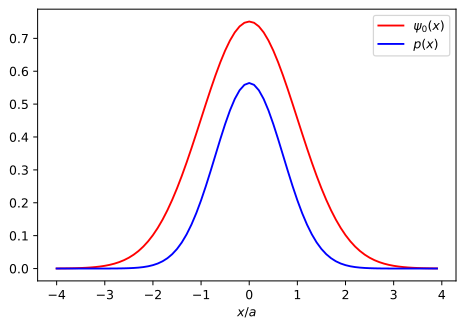
\includegraphics[scale=0.7]{ground_state.png}}
\caption{Graph showing the energy of the ground state wave function, and its probability density.}
\label{fig:ground_state}
\end{figure}
From these graphs, we can see that the ground state wave function $\psi_0(x)$ is an even function.
\subsection{Orthogonality}
To apply the position and momentum operators to the wave function, we must first verify that it is normalised and orthogonal. To verify orthogonality of normalised eigenfunctions, we use the inner product:
\begin{equation}
\bra{\psi_m} \ket{\psi_n} = \delta_{mn}
\end{equation}
Where $\delta_{ij}$ is the Kronecker delta function:
\begin{equation}
{\displaystyle \delta _{ij}={\begin{cases}0&{\text{if }}i\neq j,\\1&{\text{if }}i=j.\end{cases}}}
\end{equation}
To verify this, we use the \lstinline$integrate.quad$ method provided by Python's SciPy library. By constructing a function \lstinline$psi(x, n)$ in python, analogous to $\psi_n(x)$, we can calculate the inner product as the integral:
\begin{equation}
\bra{\psi_0} \ket{\psi_n}=\int^\infty_{-\infty}\psi_0^*(x)\psi_n(x)dx
\end{equation}
For $\psi_n(x)$ wave functions of $n=1, 3, 4, 7$.
\begin{lstlisting}
for i in [1, 3, 4, 7]:
    inner_product = integrate.quad(np.vectorize(lambda x: psi(x, 0)*psi(x, i)), -float("inf"), float("inf"))[0]
\end{lstlisting} As the wave functions are not complex, we use $\psi^*=\psi$. This numerical integration method verifies the orthogonality of the ground state wave function. The result for $\bra{\psi_m} \ket{\psi_4}$ is calculated as \lstinline$-6.106226635438361e-16$, but this is disregarded as a floating-point inaccuracy, as all other values of $n$ return precisely zero.
\subsection{Position operator}
To calculate the uncertainty of position for the wave function, we employ the position operator $\hat x=x$ to calculate the expectation value of the position observable. 
\begin{equation}
\expval x=\mel{\psi_0}{\hat x}{\psi_0}=\int^\infty_{-\infty}\psi_0^*(x)\ x\ \psi_0(x)dx
\end{equation}
We once again use the \lstinline$integrate.quad$ method in python:
\begin{lstlisting}
expectation_x = integrate.quad(np.vectorize(lambda x: psi(x, 0)*x*psi(x, 0)), -float("inf"), float("inf"))[0]
\end{lstlisting} This returns the value $\mel{\psi_0}{\hat x}{\psi_0}=0$, as we expected to obtain from the even parity of the probability density $|\psi_0(x)|^*$.
To find the position-squared expectation value, $\expval{x^2}$, we use a similar same code snippet, replacing \lstinline$x$ with \lstinline$x**2$, from which we obtain the value \lstinline$0.5000000000000012$. Again, we round this to 0.5 to account for floating point inaccuracy . By varying our value of $a$, we obtain the following values for $\expval{x^2}$.
\begin{table}[h!]
\centering
\begin{tabular}{cc}
a & $\expval x^2$ \\ \hline
1 & 0.5000000000000012  \\
2 & 0.25000000000000056 \\
3 & 0.16666666666666707
\end{tabular}
\caption{\label{tab:table}Values of $\expval x^2$ calculated using SciPy's numerical integration function.}
\end{table}

From these values, we can readily see that the expected value $\mel{\psi_0}{\hat x^2}{\psi_0} = a^2/2$ is obtained.
\subsection{Momentum Operator}
To calculate the momentum uncertainties, we now employ the momentum operator $\hat p=-i\hbar\nabla$ to calculate the momentum expectation value $\expval p$.
\begin{equation}
\expval x=\mel{\psi_0}{\hat p}{\psi_0}=-i\hbar\int^\infty_{-\infty}\psi_0^*(x)\ \frac\partial{\partial x} \psi_0(x)dx
\end{equation}
This differentiation is trivial, as the wave function is an exponential:
\begin{equation}
\frac\partial{\partial x} \psi_0(x) = -\frac x{a^2}\psi_0(x)
\end{equation}
We can then complete the integral in Python, using \lstinline$1j$ for $i$:
\begin{lstlisting}
expectation_p = -1j*hbar**2*integrate.quad(np.vectorize(lambda x: psi(x, 0)* (-x/a**2) * psi(x, 0)), -float("inf"), float("inf"))[0]
\end{lstlisting} This gives us the expected result of $\mel{\psi_0}{\hat p}{\psi_0}=0$.
To find the momentum-squared expectation value $\expval{p^2}$, we differentiate the wave function again:
\begin{equation}
\frac{\partial^2}{\partial x^2} \psi_0(x) = -\frac{x^2-a^2}{a^4}\psi_0(x)
\end{equation}
We can once again use the inner product:
\begin{equation}
\expval x=\mel{\psi_0}{\hat p^2}{\psi_0}=-\hbar^2\int^\infty_{-\infty}\psi_0^*(x)\ \frac{\partial^2}{\partial x^2} \psi_0(x)dx
\end{equation}
By modifying the previous code snippet, we can numerically calculate this integral.
\begin{lstlisting}
expectation_p_sq = -hbar**2*integrate.quad(np.vectorize(lambda x: psi(x, 0)* ( (x**2 - a**2) / a**4) * psi(x, 0)), -float("inf"), float("inf"))[0]
\end{lstlisting} From which we obtain a value of \lstinline$0.4999999999999988$, rounded to 0.5 for floating point accuracy. By once again varying our value of $a$, we can obtain a formula for $\expval{p^2}$ in terms of $a$ and $\hbar$.
\begin{table}[h!]
\centering
\begin{tabular}{cc}
a & $\expval x^2$ \\ \hline
1 & 0.4999999999999988  \\
2 & 0.10937499999999994 \\
3 & 0.03497942386831273
\end{tabular}
\caption{\label{tab:p_table}Values of $\expval p^2$ calculated using SciPy's numerical integration function.}
\end{table}

From Table \ref{tab:p_table}, we can show that $\mel{\psi_0}{\hat p^2}{\psi_0}$ matches the expected equation $\hbar^2/2a^2$.
\end{document}
